\documentclass[11pt]{beamer}
\usetheme{Warsaw}
\usepackage[utf8]{inputenc}
\usepackage{amsmath}
\usepackage{amsfonts}
\usepackage{amssymb}
\author{José Jácome}
\title{Introducción}
%\setbeamercovered{transparent} 
%\setbeamertemplate{navigation symbols}{} 
%\logo{} 
%\institute{} 
%\date{} 
%\subject{} 
\begin{document}

\begin{frame}
\titlepage
\end{frame}

%\begin{frame}
%\tableofcontents
%\end{frame}

\begin{frame}{Historia}

\begin{center}
\textbf{Pierre Simon Laplace}
\end{center}

\textit{Beaumont-en-Auge (Normandía) (1749) - París(1827)} fue un astrónomo, físico y matemático francés que inventó y desarrolló la transformada de Laplace y la ecuación de Laplace. Su trabajo se baso en la Mecánica Celeste (la cual le tomo cinco volumenes) también Ecuaciones Diferenciales y estudio de Probabilidades, fue estudiante de Jean d'Alembert, entre sus estudiantes destacan Siméon Denis Poisson y Joseph Fourier, fue conocido como el Newton de Francia, otro discípulo de él fue Napoleón.
\begin{center}
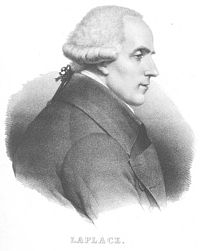
\includegraphics[scale=1.2]{Laplace.jpg}
\end{center}
\end{frame}

\begin{frame}{Introducción a la Ecuación de Laplace}
Se denomina \textit{Ecuación de Laplace} a la expresión de una ecuación en derivadas parciales de segundo orden de tipo elíptico (recordando la clasificación de las ED de segundo orden), es usado por las necesidades de la mecánica newtoniana y tiene muchas aplicación en otras ramas de la física teórica (astronomía, electrostática, mecánica de fluidos, mecánica cuántica).\\

A grandes rasgos estas EDP elípticas involucran solamente derivadas parciales respecto a variables en el espacio y, como una consecuencia, las soluciones de dichas ecuaciones están determinadas en condiciones de fronteras únicas.\\

Los tipos de EDP nos permiten describer sistemas, así las EDP elípticas (Ecuación de Laplace) permiten describir un sistema de estado estable, una EDP parabólica (ecuación de Calor) describe un sistema difuso y la EDP hiperbólica (ecuación de la Onda) describe un estado vibratorio.

\end{frame}

\begin{frame}{Deducción de la Ecuación de Laplace}

Partimos del operador Nabla.
$\displaystyle{\bigtriangledown=\hat{x} \dfrac{d}{dx}+ \hat{y}\dfrac{d}{dy}+\hat{z} \dfrac{d}{dz}}$\\ ($\hat{x},\hat{y},\hat{z}$ son los vectores unitarios)\\
Laplaciano es igual al producto escalar de nabla:
\begin{center}
$\bigtriangleup V = (\bigtriangledown \bigtriangledown)V = \bigtriangledown^{2} V  $\\
$\bigtriangledown^{2} V=(i\dfrac{dV}{dx}+j\dfrac{dV}{dy}+k\dfrac{dV}{dz}).(i\dfrac{dV}{dx}+j\dfrac{dV}{dy}+k\dfrac{dV}{dz})$\\
$\bigtriangledown^{2} V=\dfrac{d^{2}V}{dx^{2}}+\dfrac{d^{2}V}{dy^{2}}+\dfrac{d^{2}V}{dz^{2}}$
\end{center}
Igualando a cero el operador nabla obtenemos la ecuación de laplace que en coordenadas cartesianas la podemos escribir como:
\begin{center}
$\bigtriangledown^{2} V=\dfrac{d^{2}V}{dx^{2}}+\dfrac{d^{2}V}{dy^{2}}+\dfrac{d^{2}V}{dz^{2}}=0$
\end{center}
\end{frame}

\begin{frame}{Ecuación de Laplace en Coordenadas Rectangulares}
\textbf{Laplace en coordenadas Rectangulares}
\begin{center}
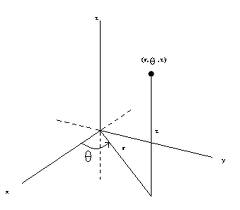
\includegraphics[scale=0.7]{rect.jpg} 
\end{center}
\end{frame}

\begin{frame}{Ecuación de Laplace en Coordenas Cilíndricas}
\textbf{Ecuación de Laplace en coordenadas Cilíndricas}\\
\begin{center}
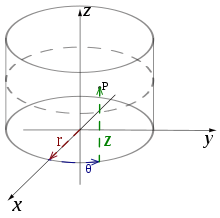
\includegraphics[scale=0.4]{esf.png} 
\end{center}
\begin{center}
$x=r.cos\phi$\\ 
$y=r.sen\phi$\\
$z=z$\\
$\dfrac{1}{r^{2}}.\dfrac{d^{2}u}{d\Theta^{2}}+\dfrac{1}{r}.\dfrac{d}{dr}(r\dfrac{du}{dr})+\dfrac{d^{2}u}{dz^{2}}=0$
\end{center}

\end{frame}

\begin{frame}{Ecuación de Laplace en Coordenadas Esféricas}
\textbf{Ecuación de Laplace en coordenadas Esféricas}
\begin{center}
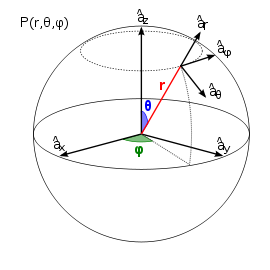
\includegraphics[scale=0.4]{cil.png} 
\end{center}
\begin{center}
$x=p.sen\Theta.cos\phi$\\
$y=p.sen\Theta.cos\phi$\\
$z=p.cos\Theta$\\
$\dfrac{1}{p^{2}}\dfrac{d}{dp}(p^{2}\dfrac{du}{dp})+\dfrac{1}{p^{2}sen\phi}\dfrac{d}{d\phi}(sen\phi.\dfrac{du}{d\phi})+\dfrac{1}{p^{2}sen^{2}\phi}.\dfrac{d^{2}u}{d\Theta^{2}}=0$\\
\end{center}

\end{frame}
\end{document}